\subsection{Kết quả thực nghiệm}

Trên cơ sở kiến trúc và các tầng bảo mật đã trình bày ở Chương~2 và Chương~3, hệ thống bỏ phiếu điện tử được hiện thực hóa thành hai sản phẩm độc lập nhưng phối hợp chặt chẽ: một \textit{ứng dụng web quản trị} dành cho ban tổ chức cuộc bầu cử và một \textit{ứng dụng di động} dành cho cử tri. Mục này trình bày kết quả thực nghiệm dưới dạng các giao diện đại diện cho toàn bộ luồng nghiệp vụ chính của hệ thống, từ khâu khởi tạo cuộc bầu cử, phân phối quyền bỏ phiếu cho đến khâu kiểm phiếu, công bố kết quả và xác minh biên lai.

\subsubsection{Giao diện phía quản trị viên (E-voting Admin)}

Ứng dụng web quản trị cung cấp các chức năng vận hành cốt lõi của một cuộc bầu cử: quản lý người dùng, khởi tạo và cấu hình cuộc bầu cử, theo dõi diễn biến bỏ phiếu thời gian thực và thực thi quy trình kiểm phiếu sau khi đóng phiếu. Giao diện được thiết kế đồng nhất theo ngôn ngữ \textit{Material Design} với bố cục dạng bảng điều khiển (dashboard) nhằm tối ưu cho thao tác nhập liệu và truy vấn dữ liệu khối lượng lớn.

Màn hình \textbf{Đăng nhập} là điểm vào duy nhất của hệ thống quản trị, yêu cầu xác thực bằng tài khoản nội bộ có gắn vai trò \textit{admin} hoặc \textit{auditor}. Phiên đăng nhập được bảo vệ bằng cơ chế JWT hai cặp khóa và lưu trữ tập trung trên Redis như đã trình bày trong Chương~3.

\begin{figure}[H]
    \centering
    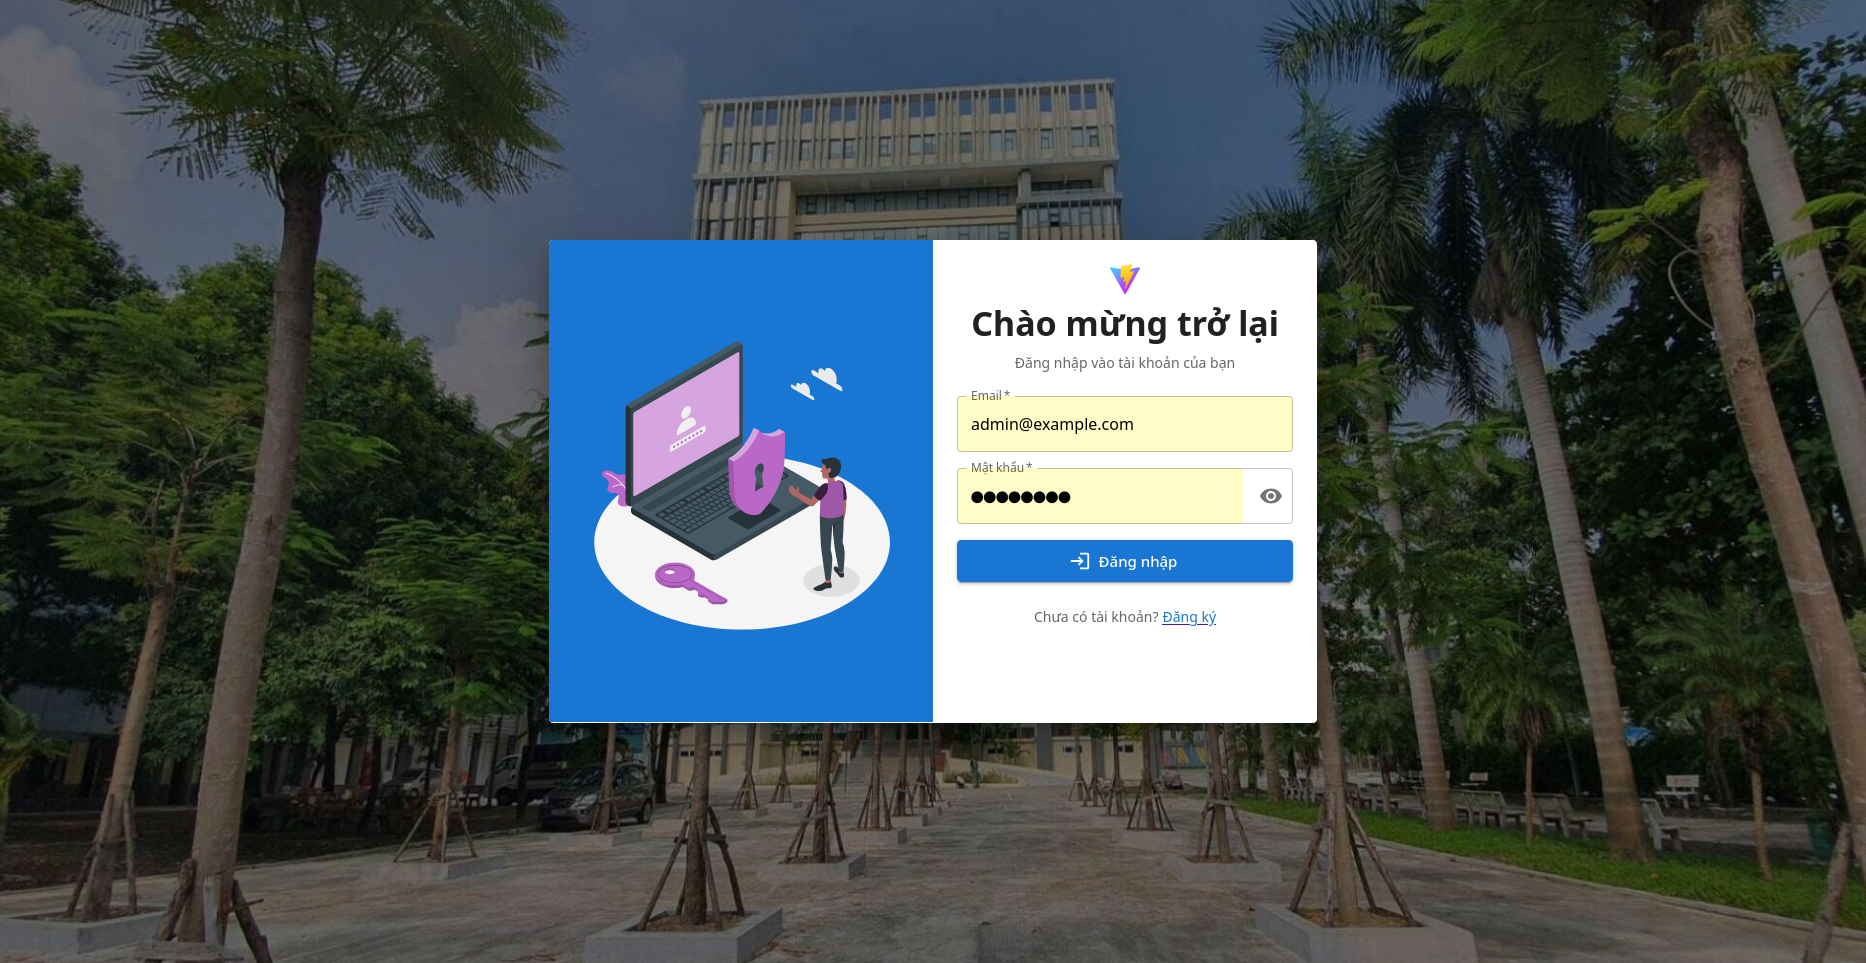
\includegraphics[width=0.85\textwidth, keepaspectratio]{Figures/Ket-qua-thuc-nghiem/Dang-nhap-E-voting-admin.png}
    \caption{Đăng nhập E-voting admin}
\end{figure}

Sau khi xác thực thành công, quản trị viên có thể truy cập \textbf{trang quản lý danh sách người dùng} để cấp quyền cử tri cho từng tài khoản, đồng bộ dữ liệu định danh và quản trị vai trò truy cập. Đây là tầng kiểm soát cử tri đầu tiên trước khi danh sách được khóa chốt cho một kỳ bầu cử cụ thể.

\begin{figure}[H]
    \centering
    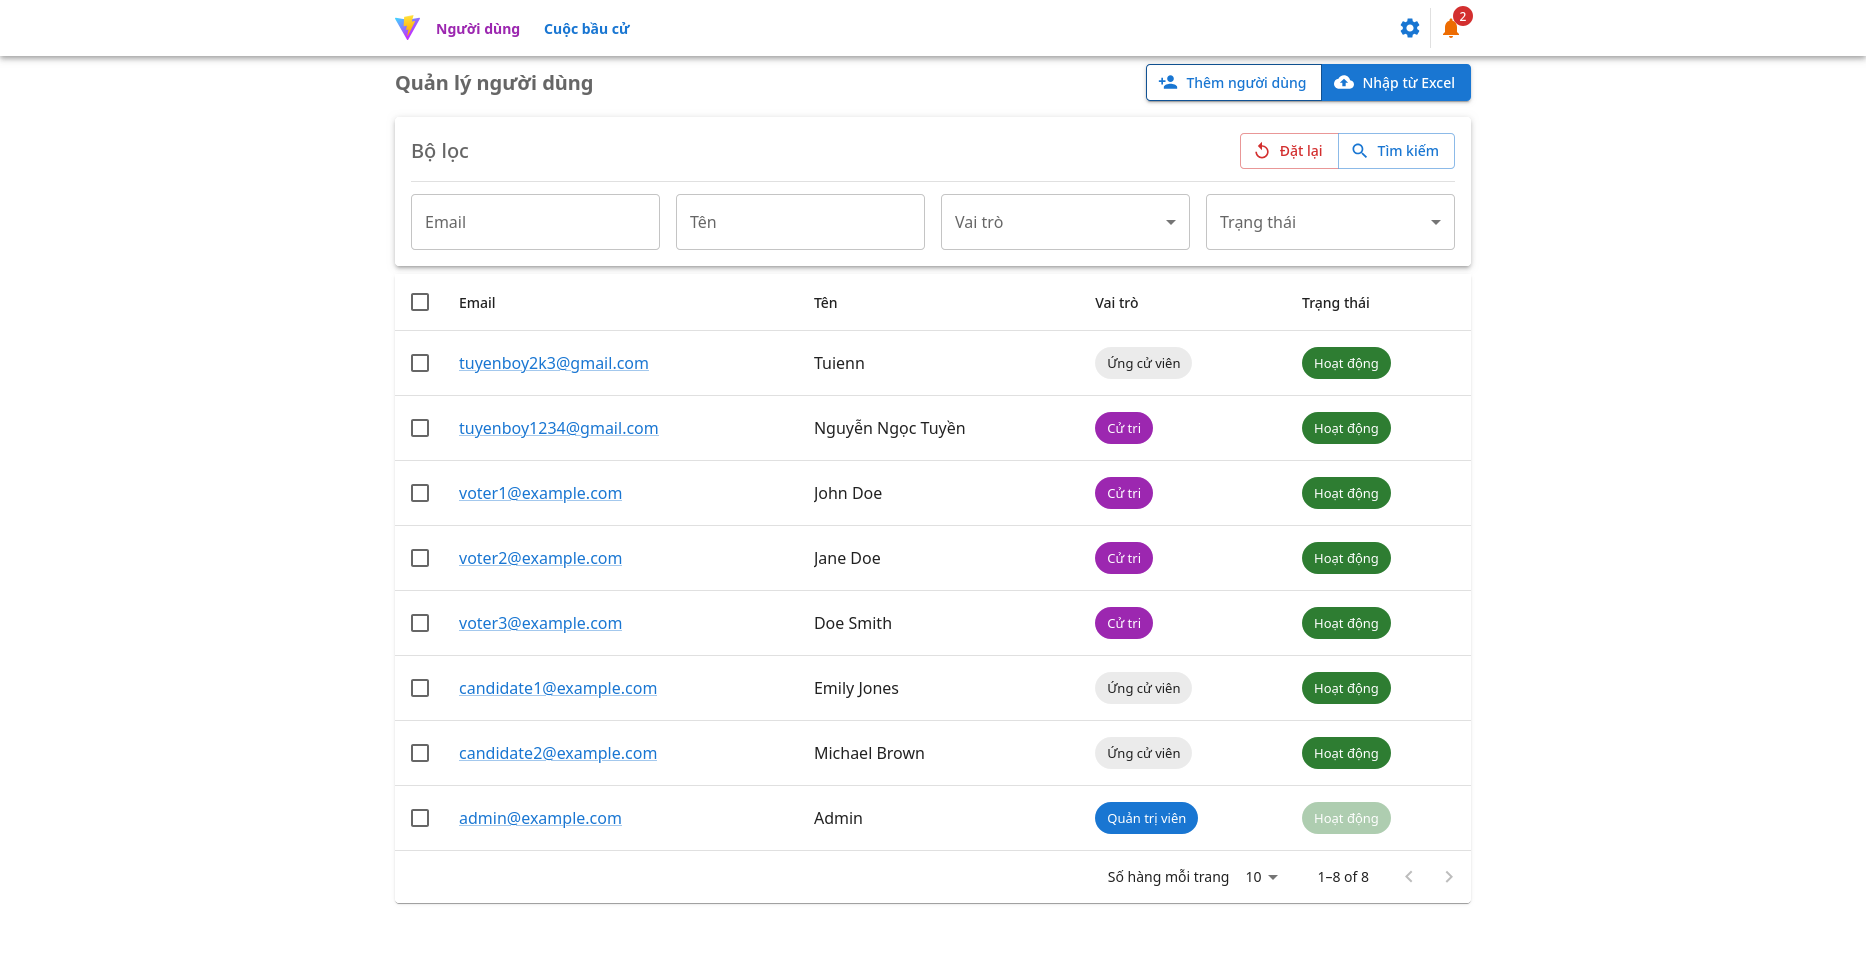
\includegraphics[width=0.95\textwidth, keepaspectratio]{Figures/Ket-qua-thuc-nghiem/Quan-ly-danh-sach-nguoi-dung-E-voting-admin.png}
    \caption{Quản lý danh sách người dùng E-voting admin}
\end{figure}

\textbf{Trang quản lý danh sách bầu cử} liệt kê toàn bộ cuộc bầu cử đã, đang và sẽ diễn ra theo từng trạng thái: \textit{nháp}, \textit{chuẩn bị}, \textit{đang diễn ra}, \textit{đã đóng phiếu}, \textit{đã công bố kết quả}. Mỗi mục cho phép truy cập nhanh tới chi tiết tương ứng để cấu hình hoặc theo dõi.

\begin{figure}[H]
    \centering
    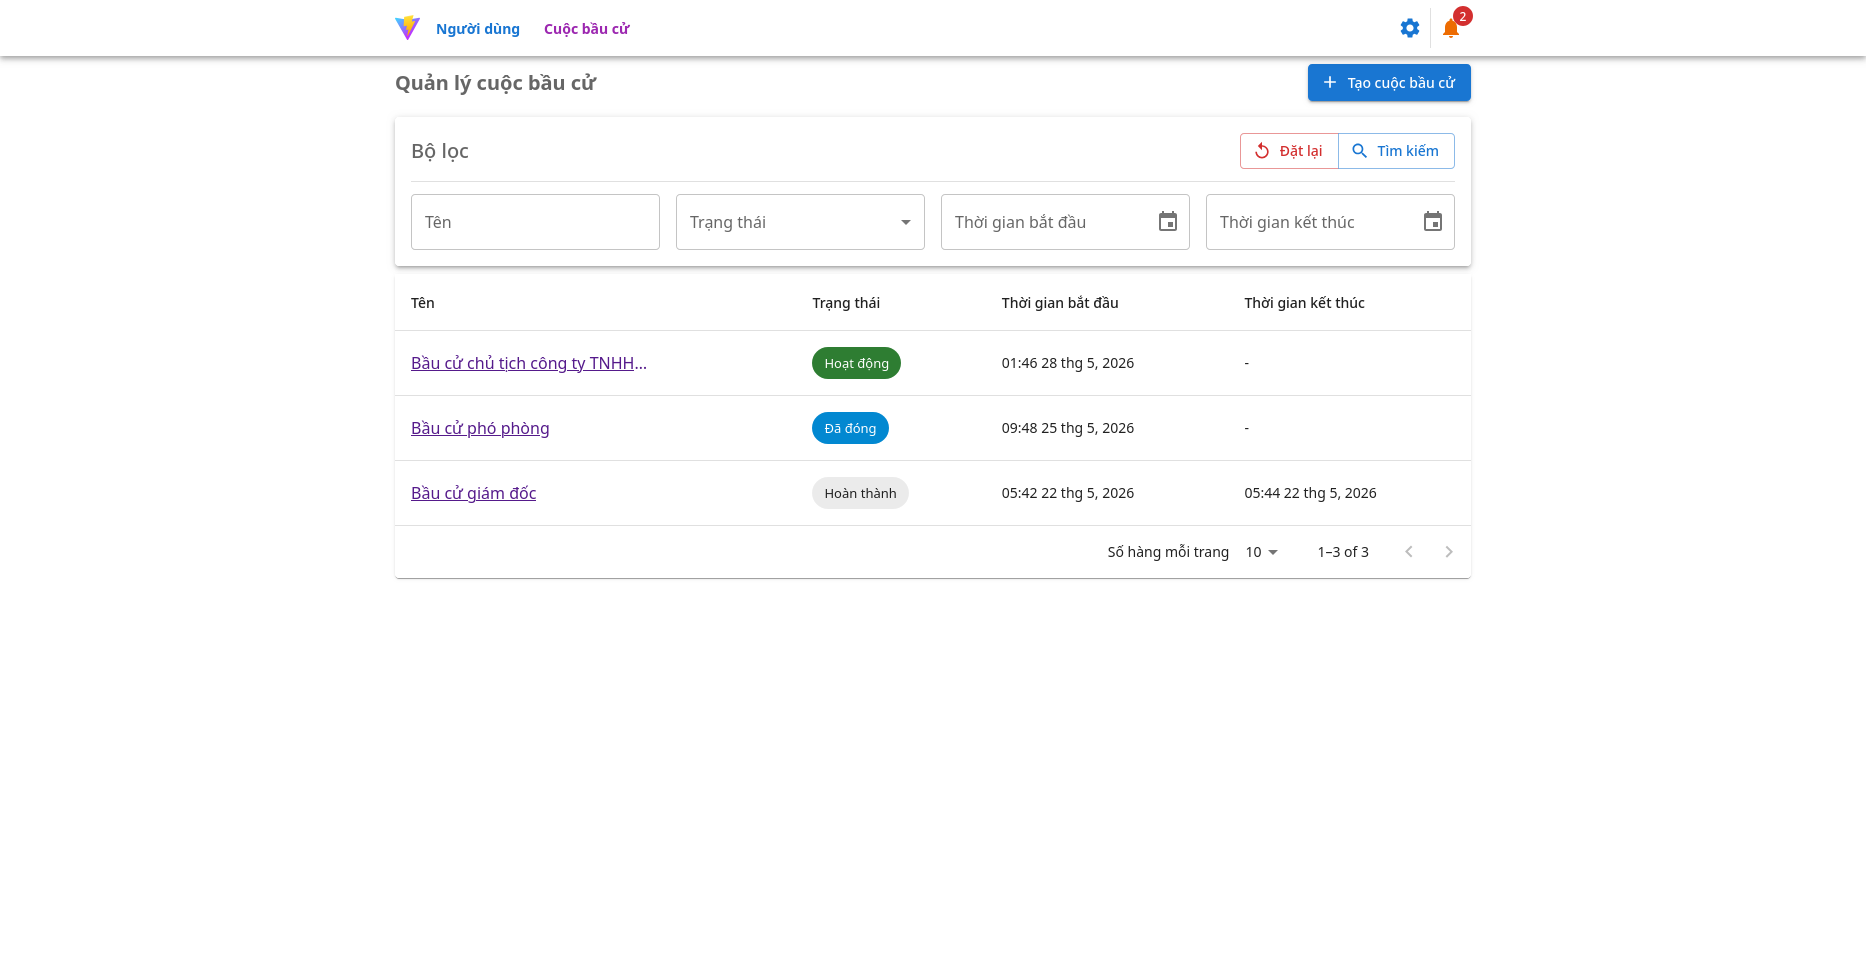
\includegraphics[width=0.95\textwidth, keepaspectratio]{Figures/Ket-qua-thuc-nghiem/Quan-ly-danh-sach-bau-cu-E-voting-admin.png}
    \caption{Quản lý danh sách bầu cử E-voting admin}
\end{figure}

Mỗi cuộc bầu cử được mô tả thông qua một trang chi tiết được chia thành nhiều tab chức năng. Tab \textbf{Thông tin cơ bản} hiển thị tên cuộc bầu cử, mô tả, mốc thời gian bắt đầu và kết thúc, danh sách ứng viên và các tham số mật mã liên quan (khóa công khai chung của bộ ký, ngưỡng $t$ trên tổng số nút ký $n$).

\begin{figure}[H]
    \centering
    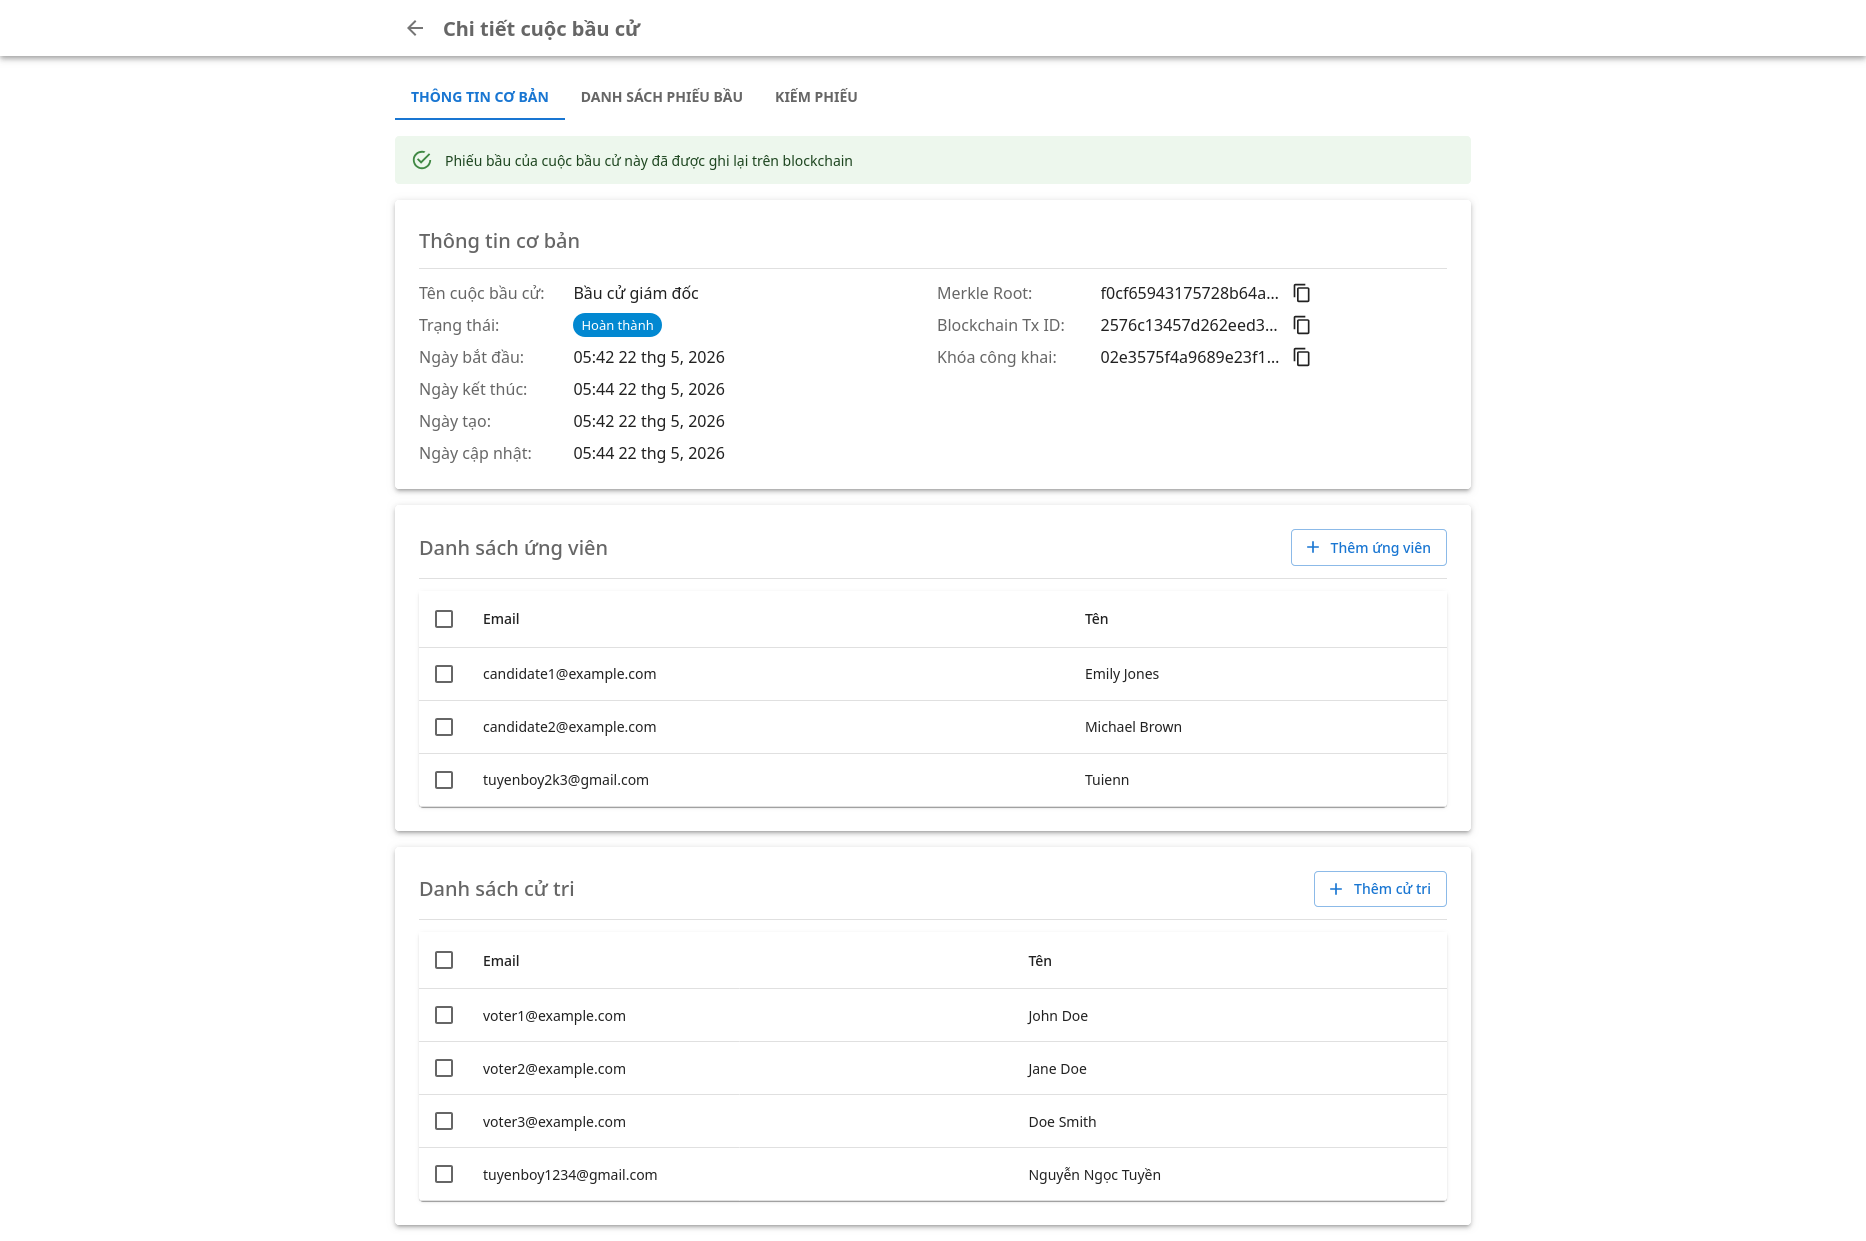
\includegraphics[width=0.95\textwidth, keepaspectratio]{Figures/Ket-qua-thuc-nghiem/Chi-tiet-cuoc-bau-cu-Thong-tin-co-ban-E-voting-admin.png}
    \caption{Chi tiết cuộc bầu cử -- Thông tin cơ bản E-voting admin}
\end{figure}

Tab \textbf{Danh sách phiếu bầu} cho phép quản trị viên và kiểm toán viên truy vấn các phiếu bầu đã được ghi nhận trên sổ cái Hyperledger Fabric. Mỗi bản ghi chỉ chứa phần dữ liệu công khai (\textit{commitment} thuộc cây Merkle, chữ ký mù tập thể, thời điểm ghi) mà không lộ danh tính cử tri, qua đó vừa cho phép kiểm chứng độc lập vừa bảo toàn tính ẩn danh.

\begin{figure}[H]
    \centering
    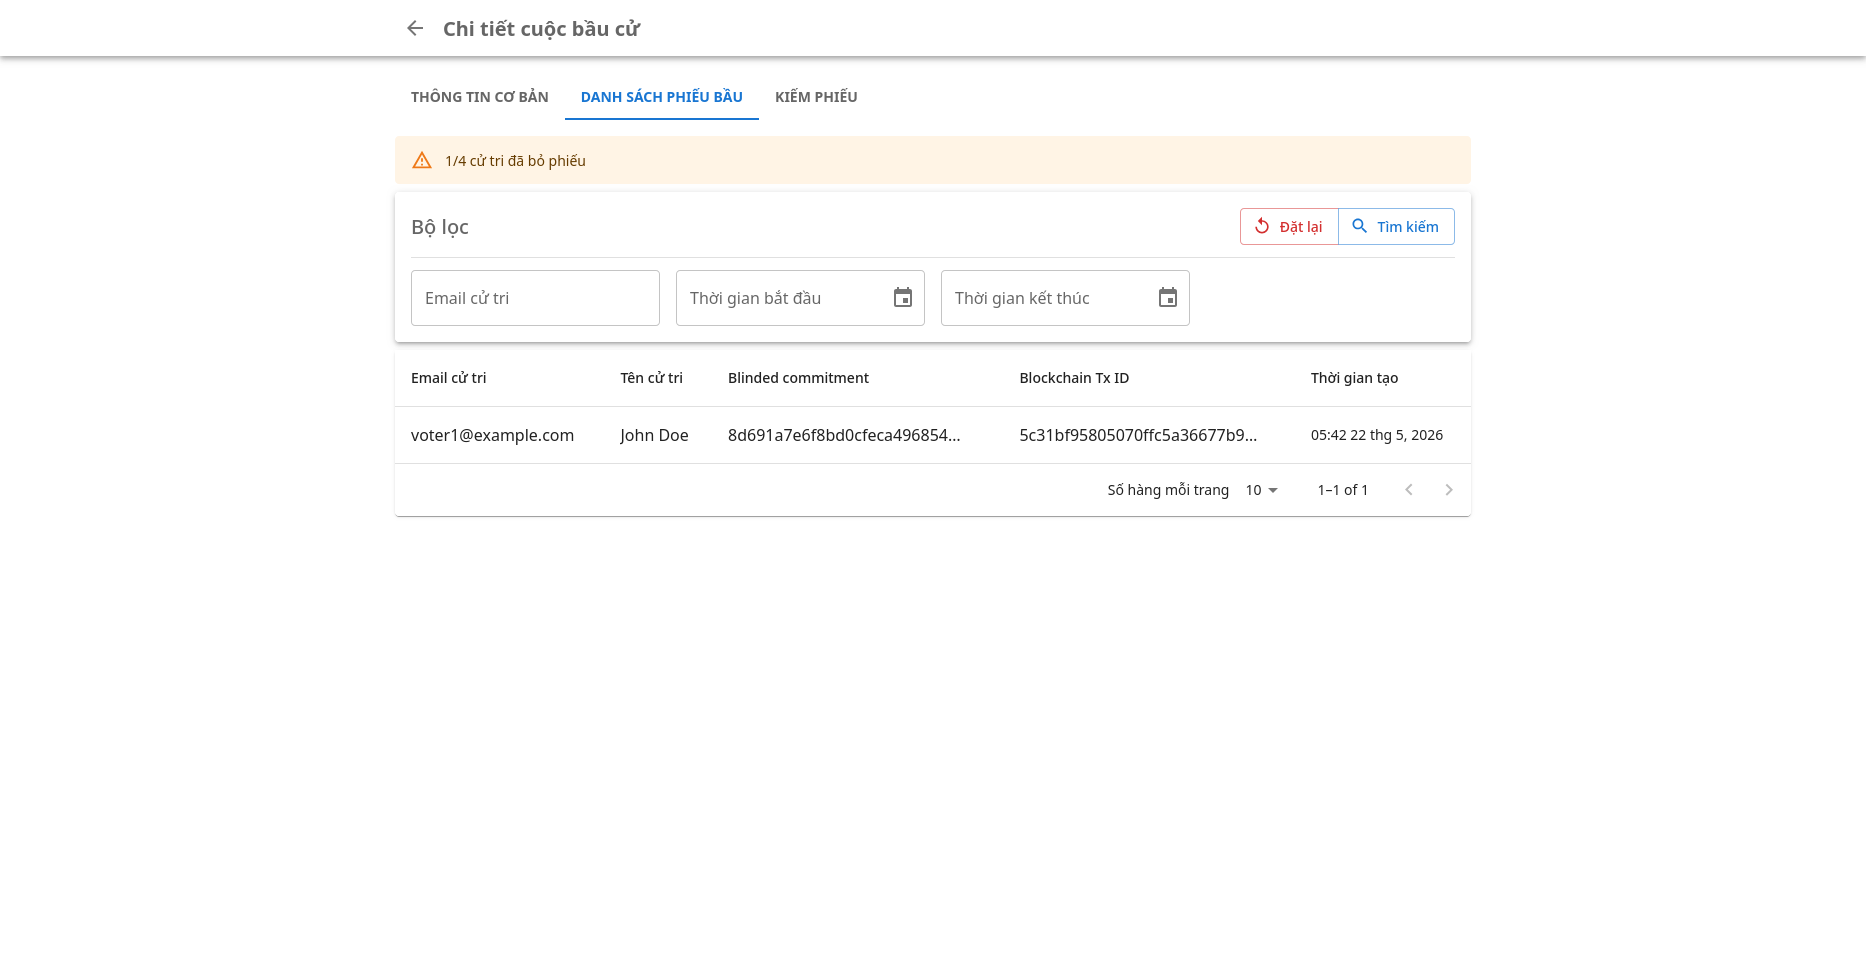
\includegraphics[width=0.95\textwidth, keepaspectratio]{Figures/Ket-qua-thuc-nghiem/Chi-tiet-cuoc-bau-cu-Danh-sach-phieu-bau-E-voting-admin.png}
    \caption{Chi tiết cuộc bầu cử -- Danh sách phiếu bầu E-voting admin}
\end{figure}

Sau khi cuộc bầu cử kết thúc, quản trị viên chuyển sang tab \textbf{Kiểm phiếu} để khởi chạy quy trình giải mã tổng hợp và đối chiếu cây Merkle. Tab này hiển thị tiến độ kiểm phiếu, tổng số phiếu hợp lệ, phiếu trùng bị từ chối và bảng phân bố kết quả theo ứng viên. Đây là điểm kết thúc quy trình quản trị ở phía máy chủ trước khi kết quả được công bố ra ứng dụng cử tri.

\begin{figure}[H]
    \centering
    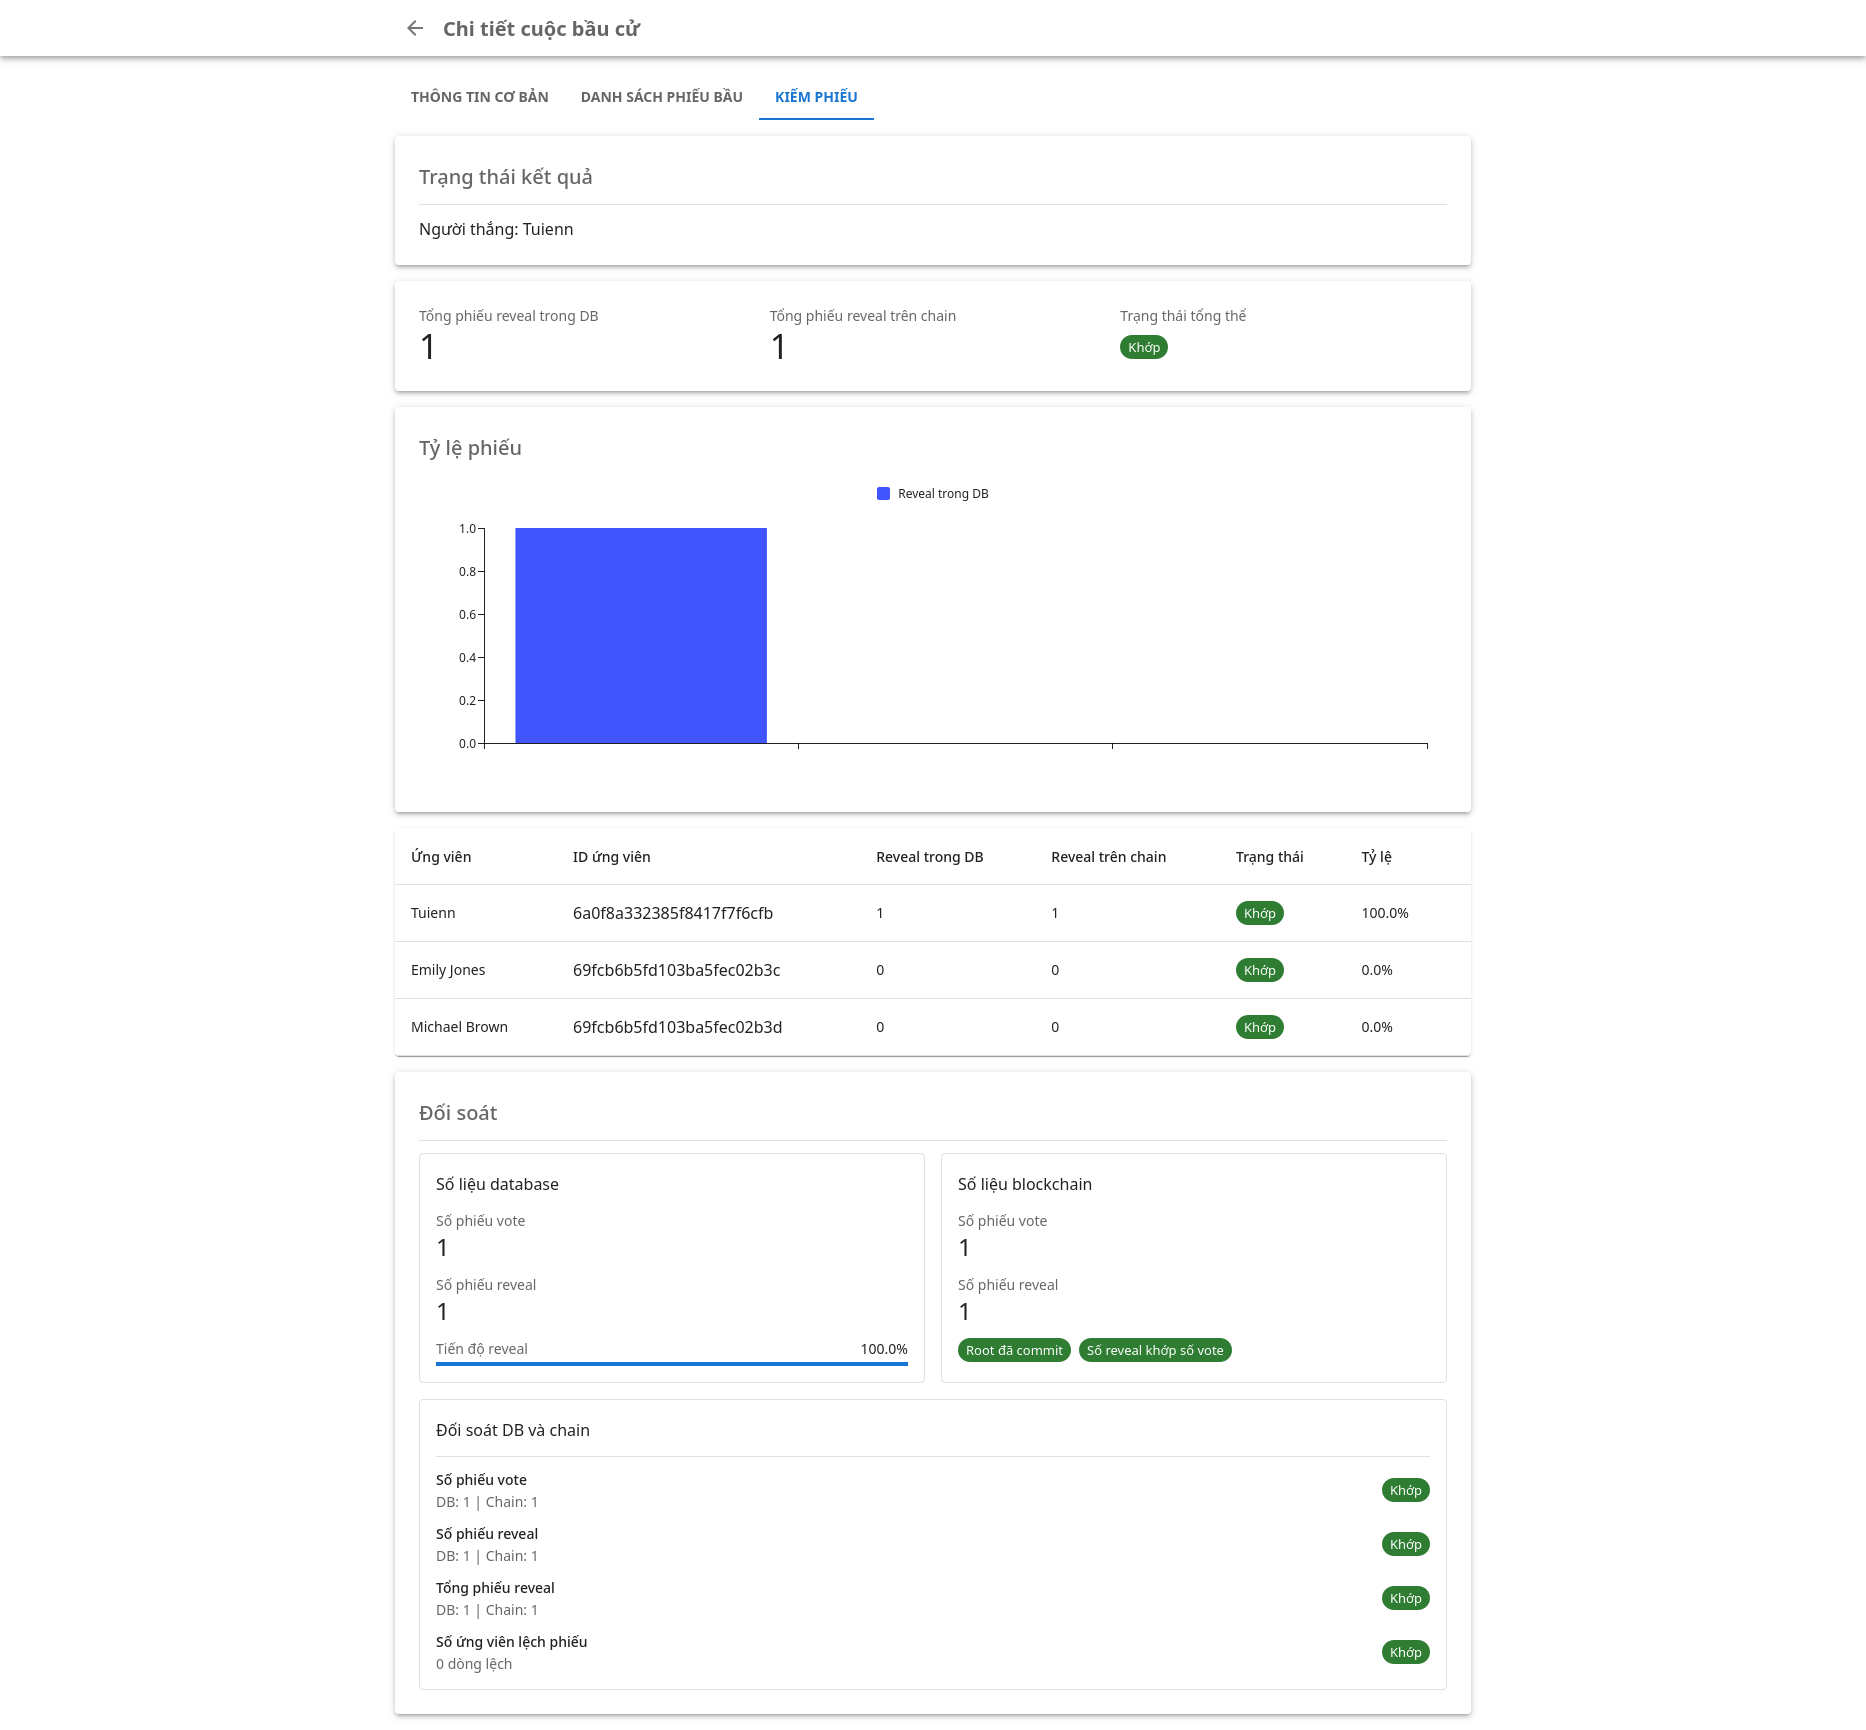
\includegraphics[width=0.95\textwidth, keepaspectratio]{Figures/Ket-qua-thuc-nghiem/Chi-tiet-cuoc-bau-cu-Kiem-phieu-E-voting-admin.png}
    \caption{Chi tiết cuộc bầu cử -- Kiểm phiếu E-voting admin}
\end{figure}

\subsubsection{Giao diện phía cử tri (E-voting Mobile)}

Ứng dụng di động được phát triển trên nền tảng Expo cho phép cử tri thực hiện toàn bộ quy trình bỏ phiếu trên thiết bị cá nhân: từ đăng nhập, lựa chọn cuộc bầu cử, thực hiện bỏ phiếu cho đến lưu giữ biên lai và tự xác minh phiếu bầu sau khi kết quả được công bố. Giao diện được thiết kế theo nguyên tắc tối giản với màn hình tập trung vào một thao tác duy nhất tại mỗi thời điểm nhằm giảm rủi ro nhầm lẫn của cử tri.

Màn hình \textbf{Đăng nhập} xác thực cử tri bằng tài khoản đã được quản trị viên cấp quyền ở phía web admin. Mỗi phiên đăng nhập thành công khởi tạo một cặp khóa cục bộ lưu trong vùng \textit{Secure Storage} của thiết bị, phục vụ ký mù phiếu bầu ở các bước sau.

\begin{figure}[H]
    \centering
    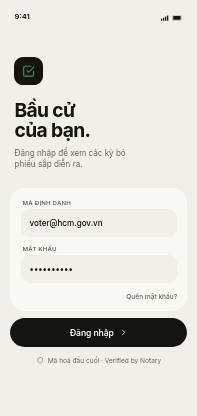
\includegraphics[width=0.45\textwidth, keepaspectratio]{Figures/Ket-qua-thuc-nghiem/Dang-nhap-E-voting-mobile.png}
    \caption{Đăng nhập E-voting mobile}
\end{figure}

Sau khi đăng nhập, cử tri được dẫn tới màn hình \textbf{Danh sách cuộc bầu cử} hiển thị các kỳ bầu cử mà tài khoản hiện tại có quyền tham gia, kèm trạng thái (sắp diễn ra, đang mở phiếu, đã đóng phiếu, đã công bố kết quả) và thời gian kết thúc đếm ngược trực quan.

\begin{figure}[H]
    \centering
    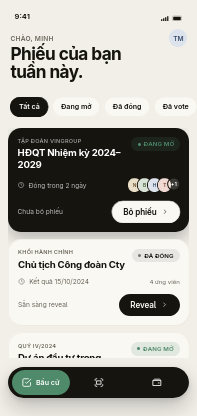
\includegraphics[width=0.45\textwidth, keepaspectratio]{Figures/Ket-qua-thuc-nghiem/Danh-sach-cuoc-bau-cu-E-voting-mobile.png}
    \caption{Danh sách cuộc bầu cử E-voting mobile}
\end{figure}

Lựa chọn một cuộc bầu cử đang mở phiếu sẽ đưa cử tri đến màn hình \textbf{Bầu cử} -- trung tâm của toàn bộ trải nghiệm. Tại đây, cử tri xem thông tin ứng viên, chọn một lựa chọn và xác nhận. Trong thao tác xác nhận, ứng dụng thực thi giao thức EC-Schnorr ký mù tập thể với máy chủ ký mà không tiết lộ lựa chọn của cử tri.

\begin{figure}[H]
    \centering
    
\includegraphics[width=0.45\textwidth, keepaspectratio]{Figures/Ket-qua-thuc-nghiem/Bau-cu-E-voting-mobile.png}
    \caption{Bầu cử E-voting mobile}
\end{figure}

Khi phiếu bầu được ghi nhận thành công lên sổ cái, hệ thống hiển thị màn hình \textbf{Bầu cử thành công} kèm mã biên lai duy nhất. Biên lai này là bằng chứng để cử tri xác minh phiếu bầu của mình đã được tính trong khâu kiểm phiếu mà không lộ lựa chọn của cử tri ra bên ngoài.

\begin{figure}[H]
    \centering
    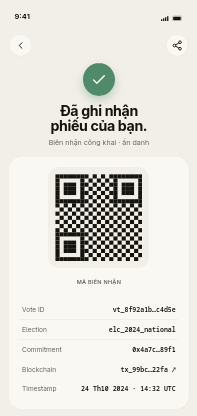
\includegraphics[width=0.45\textwidth, keepaspectratio]{Figures/Ket-qua-thuc-nghiem/Bau-cu-thanh-cong-E-voting-mobile.png}
    \caption{Bầu cử thành công E-voting mobile}
\end{figure}

Toàn bộ biên lai phát sinh từ các cuộc bầu cử mà cử tri đã tham gia được tập hợp trong màn hình \textbf{Danh sách biên lai}. Cử tri có thể truy cập lại bất kỳ biên lai nào ngay cả khi cuộc bầu cử đã kết thúc, phục vụ mục đích lưu trữ cá nhân và đối soát.

\begin{figure}[H]
    \centering
    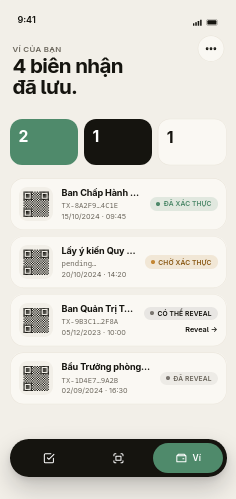
\includegraphics[width=0.45\textwidth, keepaspectratio]{Figures/Ket-qua-thuc-nghiem/Danh-sach-bien-lai-E-voting-mobile.png}
    \caption{Danh sách biên lai E-voting mobile}
\end{figure}

Khi cuộc bầu cử kết thúc và ban tổ chức công bố kết quả, cử tri có thể chủ động xác minh phiếu bầu của mình thông qua màn hình \textbf{Xác minh biên lai}. Quy trình xác minh đối chiếu \textit{commitment} của phiếu với nhánh tương ứng trên cây Merkle đã được ghi lên sổ cái Fabric; thao tác này được thực hiện độc lập, không phụ thuộc vào máy chủ vận hành.

\begin{figure}[H]
    \centering
    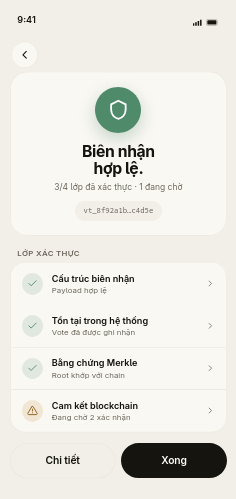
\includegraphics[width=0.45\textwidth, keepaspectratio]{Figures/Ket-qua-thuc-nghiem/Xac-minh-bien-lai-E-voting-mobile.png}
    \caption{Xác minh biên lai E-voting mobile}
\end{figure}

Song song với cơ chế xác minh từng phiếu, màn hình \textbf{Công bố phiếu} hiển thị danh sách phiếu công khai đã được ghi nhận trong cuộc bầu cử kèm các tham số mật mã cho phép bên thứ ba tự kiểm chứng tính toàn vẹn của toàn bộ tập phiếu.

\begin{figure}[H]
    \centering
    
\includegraphics[width=0.45\textwidth, keepaspectratio]{Figures/Ket-qua-thuc-nghiem/Cong-bo-phieu-E-voting-mobile.png}
    \caption{Công bố phiếu E-voting mobile}
\end{figure}

Cuối cùng, màn hình \textbf{Kết quả cuộc bầu cử} trình bày tổng kết kết quả kiểm phiếu dưới dạng biểu đồ và bảng số liệu, kèm các thông tin chứng cứ (số phiếu hợp lệ, số phiếu trùng bị loại, mã cam kết của cây Merkle cuối cùng) để cử tri đối chiếu với dữ liệu công khai trên sổ cái.

\begin{figure}[H]
    \centering
    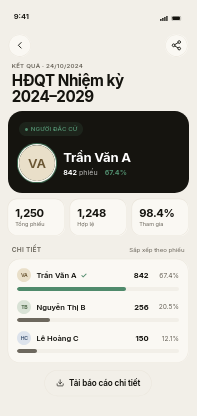
\includegraphics[width=0.45\textwidth, keepaspectratio]{Figures/Ket-qua-thuc-nghiem/Ket-qua-cuoc-bau-cu-E-voting-mobile.png}
    \caption{Kết quả cuộc bầu cử E-voting mobile}
\end{figure}
